\chapter{Experiments}
\section{Authentication Scenario:}

In the following Java example the method createDBAccess is used to create a DBAccess object for a database management application.

\begin{lstlisting}
public DBAccess createAccount(String userName, String userType,
 String userPassword) {

		DBAccess access = new DBAccess();
		access.setUserName(userName);
		access.setUserType(userType);
		access.setUserPassword(userPassword);	
				
		return access;
}

\end{lstlisting}

However, there is no authentication mechanism to ensure that the user creating this database user account object has the authority to create new user access. Some authentication mechanisms should be used to verify that the user has the authority to create database access objects.
The following Java code includes a boolean variable and method for authenticating a user. If the user has not been authenticated then the createAccount will not create the database access object.

\begin{lstlisting}

private boolean isUserAuthentic = false;

// authenticate user,
// if user is authenticated then set variable to true
// otherwise set variable to false
public boolean authenticateUser(String username, String password) {
...
}

public DBAccess createAccount(String userName, String userType,
String userPassword) {
			DBAccess access = null;
			
			if (isUserAuthentic) {
			access.setUserName(userName);
			access.setUserType(userType);
			access.setUserPassword(userPassword);
		}
	return access;
}
\end{lstlisting}

Now let's model this kind of scenario in UML statechart considering that for C/C++ application.

\begin{figure}[htbp]
	\centering
	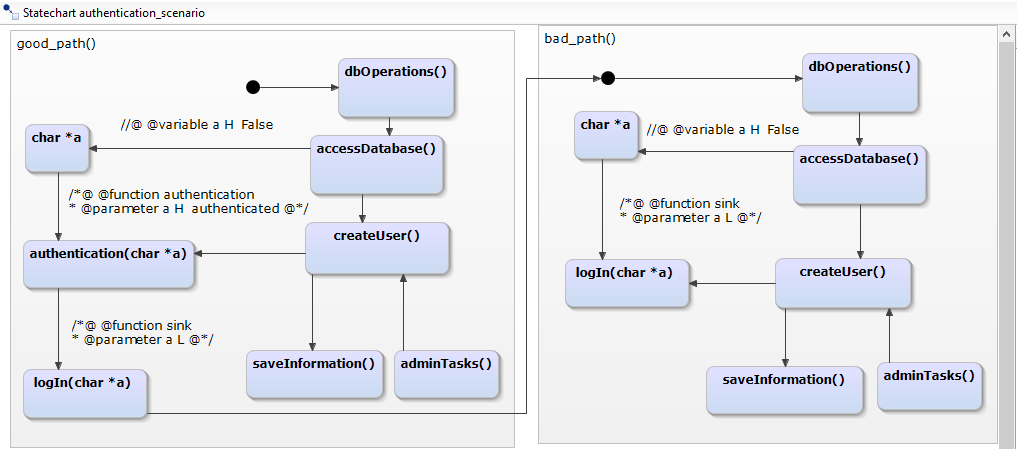
\includegraphics{styles/authentication_scenario.png}
	\caption{Authentication Scenario}
\end{figure}

\section{Declassification Scenario:}

\section{Sanitization Scenario:}